\documentclass[tikz,border=5pt]{standalone}
% ============================================================
%  style.tex
%  Style commun pour les graphes de fonctions et d'intégrales
%  Usage : \input{style.tex}  (à placer après \documentclass)
% ============================================================

\usepackage{pgfplots}
\pgfplotsset{compat=1.18}
\usepackage[T1]{fontenc}
\usepackage{amsmath,amsfonts}
\usepackage{xcolor}
\usetikzlibrary{patterns}
\usepgfplotslibrary{fillbetween}

% ---- Couleurs standard ----
\colorlet{monGris}{black!45}   
\colorlet{monBleu}{blue!60}  

% ============================================================
%  Styles TikZ (\tikzset) : tout ce qui touche à l'apparence
%  (couleurs, épaisseurs, hachures, position des étiquettes...)
%  -> utilisables aussi bien sur \node, \draw, \addplot, etc.
% ============================================================
\tikzset{
  % Courbe "secondaire" en nuance de gris (tracé + étiquette)
  courbe/.style={thick},
  % Hachures
  hachure/.style={
    pattern=north east lines,
    pattern color=#1,
    draw=none,
    samples=100,
    /pgfplots/forget plot,
  },
  hachure/.default=black,
}

% ============================================================
%  Style pgfplots (\pgfplotsset) : options propres à l'environnement axis
%  (repère orthonormé, ticks, épaisseur des axes...)
%  -> ces clés n'existent que dans /pgfplots/, \tikzset ne peut pas les définir.
% ============================================================
\pgfplotsset{
    axes/.style={
    axis lines=middle,
    axis equal image,               % repère orthonormé
    thick,                          % épaisseur des axes et courbes
    samples=200,
  }
}


\begin{document}
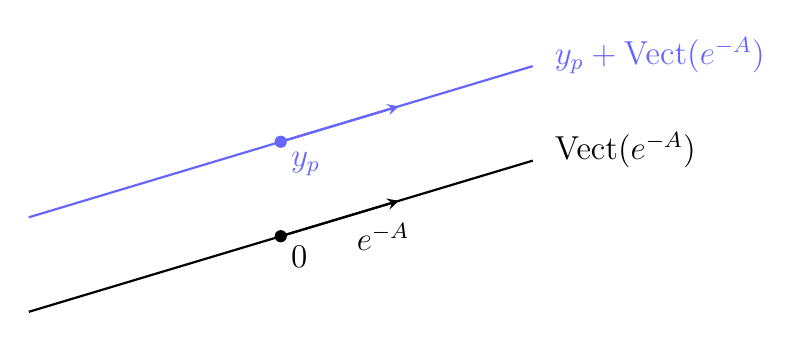
\begin{tikzpicture}[>=stealth, thick, every node/.style={font=\large}]

% Droite vectorielle des solutions de l'équation homogène (H1) : Vect(e^{-A})
\draw (-3.2,-0.96) -- (3.2,0.96);
\node[anchor=west] at (3.35,1.1) {$\mathrm{Vect}(e^{-A})$};

% Vecteur directeur de cette droite, d'origine 0
\draw[->] (0,0) -- (1.5,0.45);
\node[below] at (1.3,0.3) {$e^{-A}$};

% Origine
\fill (0,0) circle (2.2pt);
\node[below right] at (0,0) {$0$};

% Droite affine des solutions de l'équation complète (E1) : y_p + Vect(e^{-A})
\draw[monBleu] (-3.2,0.24) -- (3.2,2.16);
\node[monBleu, anchor=west] at (3.35,2.3) {$y_p + \mathrm{Vect}(e^{-A})$};

% Même vecteur directeur, même taille, sans étiquette
\draw[->, monBleu] (0,1.2) -- (1.5,1.65);

% Point y_p, étiquette au-dessus (hors de la droite)
\fill[monBleu] (0,1.2) circle (2.2pt);
\node[monBleu, below right] at (0,1.2) {$y_p$};

\end{tikzpicture}
\end{document}
